\movetooddpage
\pagebreak
\begin{center}
{\MyriadPro{\normalsize{Prefácio\\{}Livro fatídico}\\\smallskip
\small{Valéri Sájin}
}}
\end{center}
\label{prefacio}


Na primavera de 1929, em Leningrado, o almanaque \emph{A banheira de
Arquimedes} era preparado para publicação. Esse título deveria informar
ao futuro leitor de uma descoberta comparável à descoberta de
Arquimedes: ao mergulhar na leitura do almanaque, ele descobriria uma
literatura soviética inovadora e fora do comum e leria artigos dedicados
ao estudo dessa literatura. Na qualidade de pesquisadores, deveriam se
apresentar os chamados filólogos ``formalistas'', que declaravam a
necessidade do estudo da poética da literatura, de seu aspecto estético,
e não do ideológico. Quanto aos autores, foi proposta a participação de
escritores cujas obras correspondessem preferencialmente a essa
concepção: Daniil Kharms, Aleksándr Vvediénski, Nikolai Zabolótski,\footnote{Aleksándr Vvediénski (1904-1941), Daniil Kharms (1905-1942) e Nikolai Zabolótski (1903-1958) fizeram parte da Associação para uma arte real, a \emph{Oberiu}, grupo de vanguarda de Leningrado criado em 1928. (\scalebox{.8}{N}.~da~\scalebox{.8}{E}.)}
Velimir Khlébnikov e alguns outros --- em suas composições a estilística
prevalecia à ideologia ou a desprezava em absoluto. Também a Leonid
Dobýtchin foi proposto participar da \emph{Banheira de Arquimedes}.

A edição de uma coletânea experimental como essa em 1929 foi demasiado
inconveniente. Exatamente nesse ano se iniciou a ofensiva ideológica
total do poder comunista em todas as esferas da vida: desde a proibição
da celebração do ano"-novo com árvores de Natal (consideradas cerimoniais
religiosos descabidos) até a eliminação de editoras de cooperativas e
particulares e, gradualmente, a proibição de inúmeras e variadas
associações literárias --- deu"-se início nesse ano à formulação da
União dos Escritores Soviéticos unificada (e única).

Em novembro Dobýtchin enviou a Leningrado um conto que escrevera para
\emph{A banheira de Arquimedes} (era ``O retrato''), mas o almanaque não
estava destinado a sair.

Em todo caso, o conto de Dobýtchin foi impresso no fim de março do ano
seguinte na revista \emph{Construção} (\emph{Stroika}). A publicação foi
antecedida por uma nota da redação. A nota apresentava, em particular,
as pretensões ideológicas da obra de Dobýtchin naquele momento, mas pode
servir para explicar os motivos principais da recusa da edição do
almanaque para o qual ele tinha sido convidado a participar. ``(\ldots{}) se
o conto de Dobýtchin subjetivamente é muito curioso, objetivamente ---
nas condições do estado atual da literatura soviética --- assinala o
mesmo que os poemas de N. Zabolótski. Uma percepção `analítica' do
mundo que o decompõe em partes `objetais' ainda não unidas entre si
por uma ligação orgânica, o que é um atributo que contém em si o
perigo da visão de mundo fragmentada típica da burguesia.'' Na
conclusão, constatou"-se que essa ``tendência'' era característica ``de
um grupo inteiro de jovens escritores''.\footnote{\emph{Stroika}, 1930,
  n. 3, p. 7. (\scalebox{.8}{N}. do \scalebox{.8}{A}.)}

Sob a ``ligação orgânica'' das partes do mundo, da qual se falou na
referida nota da redação, subentende"-se a essência da ideologia corrente
--- essa era a exigência política imposta de forma inexorável pelo poder
à literatura soviética.

Dobýtchin não correspondia organicamente a essa exigência. E por essa
razão fora convidado para participar do almanaque dos ``formalistas''.

Até 1929 ele só havia publicado cerca de uma dezena de contos e, além
disso, cada um tinha apenas de uma a três ou quatro páginas (em toda a
sua vida criativa Dobýtchin tinha publicado dezesseis contos, e o maior deles
com muito custo alcançou oito páginas). Que características os autores
da \emph{Banheira de Arquimedes} viram nos textos reduzidos de Dobýtchin
que seriam condizentes com a apresentação de uma literatura soviética
fora do padrão, inovadora?

Vamos recorrer a uma comparação.

Nesse mesmo almanaque teriam sido publicados, entre outros, contos de
Daniil Kharms. Como este, por exemplo: ``Um bonde vem vindo. Há oito
passageiros no bonde. Três estão sentados: dois à direita e um à
esquerda. E cinco estão de pé e seguram"-se em alças de couro: dois à
direita e três à esquerda. As pessoas do grupo sentado olham umas para
as outras e as do grupo de pé estão de costas umas para as outras. Ao
lado a cobradora está de pé em cima de um banco (\ldots{})''. E assim por
diante. Aqui (e em várias outras miniaturas de Kharms que ocupam às
vezes metade de uma página) significativamente há ausência de enredo com
desenlaces motivados de uma ou de outra maneira e eliminação total de
reflexão, seja do autor seja da personagem. Era realmente uma ``outra''
prosa que se distinguia essencialmente da literatura russa tradicional
--- do manual da vida, da literatura que se ocupa da resolução de
``problemas eternos'' e da busca de respostas a ``questões malditas''.

Quanto a esse aspeto a prosa de Dobýtchin se mostra particularmente
próxima da prosa de Kharms. ``Velhas senhoras arrastavam"-se com
vassourinhas de banho e toalhas amarradas na cintura. Crostas de neve
estalavam. Escurecia. Lampiões ardiam sem brilho. Um pequeno sino
tilintou: Málkina, funcionária do Jenotdel, olhando de vez em quando
para os transeuntes, saía em missão. Sentada num banquinho alto, a
inválida Katz, imponente, concluía a venda de um pãozinho doce. O
agulheiro assoprou a corneta. A entrada da ponte afastava"-se para a
escuridão, e de lá, reluzindo, uma faísca aproximava"-se.''
(``Konopátchikova'')\footnote{\scalebox{.8}{DOBÝTCHIN}, Leonid. Konopátchikova.
  \emph{Encontros com Liz e outras histórias.} Tradução: Moissei
  Mountian. São Paulo: Kalinka, 2009, p. 74. (\scalebox{.8}{N}.~da~\scalebox{.8}{E}.)} Ou: ``Igrejas
se erguiam. Ruas desciam e subiam. Velhos sentavam"-se nos aterros em
volta das casas. Goteiras cintilavam e, ao caírem nos ombros,
respingavam. Como sempre, na esquina, meu pai se despediu com um toque
na aba do chapéu''. (``O retrato'')\footnote{\emph{Ibid.}, p. 127. (\scalebox{.8}{N}.
  da \scalebox{.8}{E}.)}

De forma análoga ao que ocorrera na segunda metade do século \scalebox{.8}{XIX},
quando, em oposição à literatura didática enraizada na Rússia da época,
surgira a assim chamada poesia ``pura'' (Afanássi, Fet, Apollón Máikov e
outros), na Rússia soviética dos anos 1920, em oposição à literatura de
propaganda incentivada pelo governo, formou"-se uma prosa
``contemplativa'', empenhada em fazer observações atentas sob o fluxo
contínuo da vida e em reproduzi"-la em detalhes ínfimos, fisgados pelo
olhar perscrutador do escritor.

Dobýtchin era um desses poucos --- devido às circunstâncias do período
--- contempladores atentos do mundo. Seu mundo era o espaço da pequena
província (sem dúvida Briansk, com uma população de oitenta e poucos mil
habitantes, onde ele vivera) de onde ele transfere os topônimos
meticulosamente fixados de conto em conto e, o principal, acontecimentos
semelhantes. Em cada um de seus contos invariavelmente aparecem feriados
soviéticos altivos acompanhados por orquestra (o Dia Internacional de
Solidariedade aos Trabalhadores, em 1º de maio, ou o dia da Revolução de
Outubro, em 7 de novembro) e, em paralelo, volta e meia executam ofícios
religiosos, enterros com missas fúnebres ou a leitura do Evangelho por
uma ou outra personagem. Esses eventos mínimos e estereotípicos,
justapostos no espaço microscópico do texto, com diluição do enredo e
sem manifestação ética (muito menos ideológica) da posição do autor,
definem o estilo inconfundível do escritor Dobýtchin.

Ele assim entrou na vida pública: no fim do verão de 1924 remeteu dois
contos ao acaso para a revista leningradense \emph{O contemporâneo
russo} (\emph{Rússkii sovremiénnik}) e eles foram quase que imediatamente publicados.

Dobýtchin caiu em boas mãos. Foi apadrinhado por escritores não
estranhos a inovações literárias (por vezes oficialmente): Kornei
Tchukóvski e seu filho Nikolai, Mikhail Slonímski, Veniamin Kaviérin e
outros prosadores de Leningrado. Eles aceitaram e incentivaram o estilo
distanciado de Dobýtchin, contribuíram para a publicação de seus contos
e para a apresentação do escritor em dezembro de 1929 na União dos
Escritores de Toda a Rússia. Mas vez ou outra censuravam a brevidade,
assim a julgavam, de suas obras e insistiam para que ele escrevesse um
romance (por algum motivo justamente um romance). Dobýtchin tentava
corresponder aos desejos de seus protetores. De 1926 a 1932 ele de
tempos em tempos lhes informava que estava ``terrivelmente empenhado''
em escrever um romance, mas logo reconhecia com tristeza que não passava
das ``700 palavras''. Para Dobýtchin o problema consistia na visível
limitação do espaço físico de sua existência (a provinciana Briansk) e
--- como se depreende de seus contos fartos de realidades concretas ---
em sua aversão absoluta à ``invenção''. Com esse paradigma como seria
possível encontrar material para a criação de uma obra volumosa e
orgânica?

O escritor o achou em seu passado: nas recordações de sua própria
infância.

Dobýtchin nasceu em 5 (17 no calendário gregoriano) de junho de 1894. Desde os dois anos passou a
viver com os pais na Rússia ocidental, na cidade de Dvinsk, parte da
província de Vítebsk (em dezembro de 1917 os bolcheviques transferiram a
cidade para a Letônia soviética e em 1920 a nomearam Daugavpils). Aos
oito anos Leonid perdeu o pai, que trabalhava como médico. Sua mãe, que
havia concluído o Instituto de Obstetrícia em Petersburgo, cuidava da
família, mas, depois da morte do marido, viu"-se obrigada a trabalhar
como parteira. Em 1911, ao concluir a \emph{escola real} de Dvinsk,
Leonid ingressou no Departamento de Economia do Instituto Politécnico de
Petersburgo. Sua especialidade tornou"-se a estatística. Na primavera de
1918, algum tempo depois de sua mãe ter se mudado de Dvinsk para
Briansk, Dobýtchin aqui se estabeleceu e praticamente até o final de sua
vida --- com intervalos --- trabalhou em diversos institutos de estatística
da cidade.

Em maio de 1933 Dobýtchin finalmente enviou a Leningrado alguns dos
primeiros capítulos do ``romance''. Eles só puderam ser publicados
exatamente um ano depois, no quinto número (maio) da revista \emph{Terra
virgem vermelha} (\emph{Krásnaia nov}). Os treze capítulos da obra nova
--- e insolitamente grande para os leitores familiarizados com a prosa
de Dobýtchin --- receberam um título ``de gênero'' incomum: ``O início
de um romance''. Um ano e meio depois, em novembro/dezembro de 1935, com
o acréscimo de vinte e um novos capítulos ao anterior ``O início de um
romance'', o livro de Dobýtchin saiu já com o título \emph{A Cidade Ene}
(importante: sem indicação do gênero da obra). Era uma narrativa
autobiográfica sobre sua infância em Dvinsk.\footnote{O livro foi
  dedicado a um vizinho de Dobýtchin de um apartamento em Leningrado (no
  edifício 62 às margens do rio Moika), Aleksándr Pávlovitch Drozdóv. Em
  1934 se estabeleceu uma amizade intensa e fora do padrão entre
  Dobýtchin e Drozdóv. (\scalebox{.8}{N}. do \scalebox{.8}{A}.)}

Os trinta e quatro capítulos de \emph{A Cidade Ene} reproduzem em
detalhes exatamente dez anos da vida do autor"-narrador: dos seis aos
dezesseis anos de idade. A série de acontecimentos mencionados permite
inferir a extensão temporal do texto, de 1901 a 1911: no capítulo onze
se descreve uma exposição agrícola (ela ocorrera em 1903 em Dvinsk);
depois se mencionam o início da guerra com o Japão (1904) e sua
conclusão (agosto de 1905); a revolução na Turquia (1908); em seguida o
centenário do nascimento de Gógol (março de 1909); a morte de Lev
Tolstói (7 de novembro de 1910); o voo do aviador Serguei Útotchkin, que
sobrevoou Dvinsk pela primeira vez em 1º de junho de 1911\ldots{} No
intervalo entre os eventos enumerados, é mencionada uma quantidade
enorme de acontecimentos locais de Dvinsk, da Rússia e do exterior que
estão impregnados na trama historicamente precisa da \emph{Cidade Ene}
(com raros deslocamentos cronológicos).

Uma questão pode parecer estranha: em que \emph{A Cidade Ene} se
diferencia das obras conhecidas anteriores de Dobýtchin? A resposta deve
ser simples: no volume e na ausência do farto contexto soviético,
impossível em uma narrativa com episódios do comecinho do século \scalebox{.8}{XX}. Com
efeito. O paradoxo de \emph{A Cidade Ene} no entanto consiste no fato de
que a nova obra de Dobýtchin reproduz em minúcias os procedimentos
principais de suas miniaturas precedentes. Se antes eles estavam
diluídos em uma dezena de textos, agora aparecem de forma concentrada.

Da mesma forma que Dobýtchin em seus contos assinalou escrupulosamente
os topônimos no espaço em que se desenrolava a ação, em \emph{A Cidade
Ene} o leitor praticamente em cada capítulo é informado exatamente onde
e em que momento a ação se desenrola ou quais objetos se encontram no
campo de visão do menino"-narrador: o castelo"-prisão, a fortaleza
militar, o teatro e o cinema, a estação e a rua ``dos prazeres'' nos
arredores da estação, o viaduto sobre a estrada de ferro para a passagem
de uma parte da cidade à outra\ldots{} São elementos reais de Dvinsk, e
nenhum deles, ao que parece, escapou à narrativa de Dobýtchin.\footnote{Aleksándr
  Beloússov, filólogo petersburguês, chamou \emph{A Cidade Ene} de
  ``pequena enciclopédia de Dvinsk'': ele comentou escrupulosamente
  todos os topônimos mencionados no livro e os eventos históricos, e
  determinou os protótipos reais de mais de cinquenta personagens do
  livro de Dobýtchin (cf.: \scalebox{.8}{DOBÝTCHIN}, Leonid. \emph{Gorod En.}
  Daugavpils, Saule, 2007, pp. 119--226 [Bibliotheca Latgalica]). (\scalebox{.8}{N}. do
  \scalebox{.8}{A}.)}

Com eles se conjugam motivos religiosos, característicos dos eventos de
praticamente todos os contos de Dobýtchin. Em \emph{A Cidade Ene}, temos
as menções obrigatórias aos templos católicos (\emph{kostiol}), às
catedrais ortodoxas, às igrejas luteranas e aos templos dos \emph{velhos
crentes} (Dvinsk era uma cidade multinacional e multiconfessional), e,
quando a ação por vezes se desloca da cidade natal do menino para outro
espaço, inevitavelmente se indicam os templos locais. Além disso, com
frequência, de capítulo em capítulo (em vinte e nove dos trinta e
quatro!), são descritos ritos e festejos religiosos, e não apenas uma
vez é citado o Novo Testamento (por sinal, Dobýtchin o citava largamente
em suas correspondências)\ldots{} Pode"-se dizer que toda a vida do narrador,
de uma ou de outra maneira, está mergulhada nessa atmosfera religiosa.

Como é evidente, nos enredos dos contos de Dobýtchin sistematicamente
surge a morte de uma ou de outra personagem, e nos enterros (ou nos
feriados) tocam orquestras. Em \emph{A Cidade Ene} o leitor desde o
começo ``escuta'' uma orquestra militar e depois, de capítulo em
capítulo, orquestras acompanham a narrativa.~O mesmo ocorre quanto aos
funerais e cemitérios: a partir do segundo capítulo, mortes, funerais e
cemitérios são circunstâncias invariáveis da vida do menino.

O caráter ``literocêntrico'' um pouco velado de seus contos
(menção a Nikolai Gógol em ``Sávkina'', a Oscar Wilde e Upton Sinclair
em ``Dorian Gray'', a Serguei Essiénin em ``O retrato'', e aparições
frequentes de bibliotecas ou ``bibliotecárias'' em vários contos) é
solidamente acentuado em \emph{A Cidade Ene}. Isso se expressa por meio
de referências contínuas a nomes e a obras de escritores russos e
estrangeiros (praticamente vinte, contando por alto) feitas pelo
narrador"-bibliófilo, que ``não tinha assunto'' com alguém de sua idade
que não lesse. E, o principal, o motivo que perpassa o livro é dado já
no título. \emph{A Cidade Ene} é o espaço gogoliano de \emph{Almas
mortas.} A personagem principal de Dobýtchin faz sistematicamente
ligações com o poema de Gógol e volta e meia se identifica com o herói
Tchítchikov, desejando mudar"-se para a formidável cidade Ene (\emph{N}
em Gógol). O que o atrai? O exemplo da amizade terna de Tchítchikov e
Manílov e o desejo de tornar"-se amigo dos filhos de Manílov.

Pode"-se dizer que, por trás do número enorme de personagens, topônimos,
fatos históricos e outros detalhes da história narrada por Dobýtchin em
\emph{A Cidade Ene}, está o relato de uma busca comovente e incansável de
uma criança por um amigo.

Nesse ponto tocamos em uma diferença fundamental entre essa obra de
Dobýtchin e seus contos.~Análogo a eles, ao longo de \emph{A Cidade Ene}
prevalece o tom neutro"-distanciado e não emotivo. Com exceção das
autorreflexões cíclicas do menino"-narrador: ``Que encantador --- pensava
eu amorosamente''; ``Fiquei comovido''; ``Eu também estava feliz'';
``Comovido, meu olhar foi atraído para as feridas de Jesus Cristo'',
``Tremendo, eu saí de casa''\ldots{} Essas autoconfissões (e outras
semelhantes) --- uma transgressão rara de Dobýtchin do estilo que
caracteriza todas as suas demais obras --- fazem alusão a uma
particularidade da personalidade e da psicologia do escritor. E podem
ser uma provável explicação para seu destino trágico.

Um mês ou um mês e meio depois de o livro ter sido impresso, em 19 de
janeiro de 1936, na Casa V. V. Maiakóvski em Leningrado, realizou"-se,
como indicado no convite, ``o sarau criativo L. I. Dobýtchin''. No
programa constava a leitura do novo livro \emph{A Cidade Ene.} Aqui os
conhecidos de Dobýtchin que apreciavam seu estilo inovador deram o tom,
e por isso, após mencionar que ele tinha alcançado ``uma harmonia entre
seu estilo e o material'', apenas recomendaram gentilmente que ``saísse
do beco do esteticismo estreito''. Ao mesmo tempo, desabaram sobre ele críticas
``ofensivas'' afirmando que o livro era ``ruim'' e ``desnecessário''.

Em 28 de janeiro, 6 de fevereiro e 1º de março, no \emph{Pravda}, o
principal jornal comunista, saíram artigos, um atrás do outro, que,
baseando"-se em exemplos negativos concretos (ópera, balé, artes
plásticas), convocavam para a luta total contra o formalismo sem
ideologia. Foi o sinal para que todas as uniões artísticas começassem a
erradicar os ``formalistas'' de seus meios.

Com esse fim, a União dos Escritores de Leningrado realizou em 25 de
março uma reunião geral chamada ``A luta do formalismo e o
naturalismo''. O tom do debate foi dado pelo crítico literário Efim
Dóbin, que, numa comunicação minuciosa, ao lado de outros textos
``condenáveis'', caracterizou \emph{A Cidade Ene} de Dobýtchin como uma
obra religiosa que cultuava um passado reacionário e perdido e por
princípio profundamente hostil ao poder soviético. Ofendido, Dobýtchin
não guardou silêncio. Fez uma breve intervenção: ``Para mim é inesperado
e lamentável que meu livro seja considerado um inimigo da classe'', e
abandonou a reunião.

No dia seguinte ele enviou a sua mãe em Briansk algumas de suas coisas.
Saldou pequenas dívidas que tinha com pessoas variadas. Sobre a mesa de
seu quarto espalhou livros pegos em lugares diferentes com instruções
sobre quem deveria recebê"-los de volta. Na manhã de 28 de março entregou
as chaves do apartamento ao seu amigo. E desapareceu.

Sem demora, quando o desparecimento de Dobýtchin tornou"-se evidente,
organizaram buscas oficiais. Mas não deram resultado. \emph{A Cidade
Ene} tornou"-se seu último --- fatídico --- livro.


\begin{flushright}
\emph{(Texto traduzido do russo)}
\end{flushright}
%\emph{Valéri Sájin}

\pagebreak
\thispagestyle{empty}

\vspace*{7.3cm}\hspace*{-3.2cm}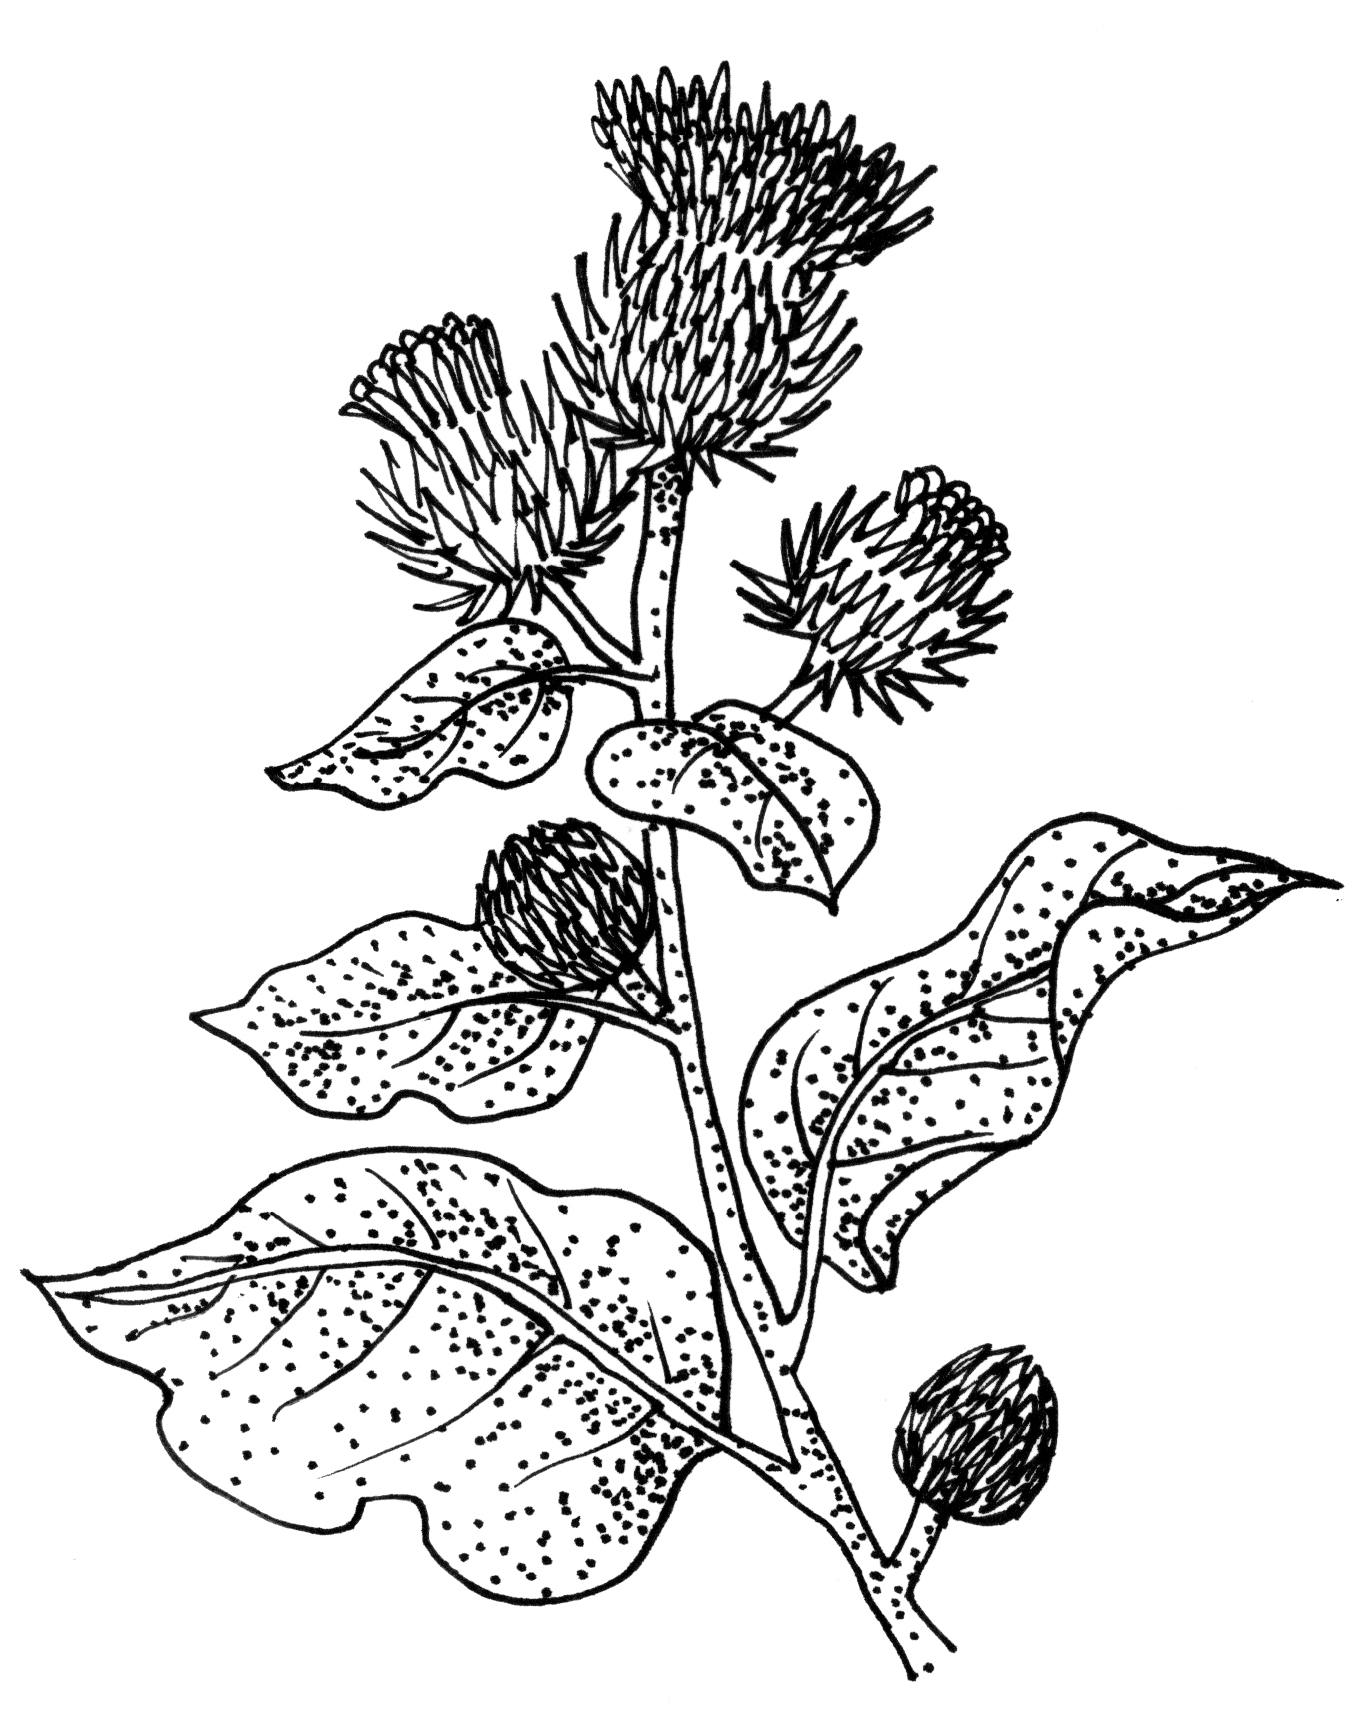
\includegraphics[width=14.7cm]{./bordo.pdf}


\pagebreak
\thispagestyle{empty}

\begin{vplace}[60]
\begin{centering}
{\small{
Os nomes e termos russos foram transliterados conforme padrão adotado pela \scalebox{.8}{USP}. Os nomes e as expressões de origem alemã, polonesa e francesa em geral seguem grafia original de cada país, no entanto em algumas ocorrências, que pareciam carregar marcas de fala, foram transliterados conforme se apresentam no romance, em que foram sempre russificados, ou seja, transliterados para o cirílico conforme a pronúncia. Feriados religiosos foram grafados em caixa"-baixa, conforme o texto seguido pela tradução. As notas de rodapé são do tradutor com colaboração da edição.
}}
\end{centering}
\end{vplace}
\thispagestyle{empty}